%%%%%%%% ICML 2018 EXAMPLE LATEX SUBMISSION FILE %%%%%%%%%%%%%%%%%

\documentclass{article}

% Recommended, but optional, packages for figures and better typesetting:
\usepackage{microtype}
\usepackage{graphicx}
\usepackage{subfigure}
\usepackage{booktabs} % for professional tables

% hyperref makes hyperlinks in the resulting PDF.
% If your build breaks (sometimes temporarily if a hyperlink spans a page)
% please comment out the following usepackage line and replace
% \usepackage{icml2018} with \usepackage[nohyperref]{icml2018} above.
\usepackage{hyperref}

\usepackage{amsmath, amsthm}
\usepackage{amsfonts}
\usepackage{amssymb}
\usepackage{comment}
\usepackage[round]{natbib}
\usepackage[dvipsnames]{xcolor}
\usepackage{array}
\usepackage{enumitem}
\setlist{nolistsep}

% Attempt to make hyperref and algorithmic work together better:
\newcommand{\theHalgorithm}{\arabic{algorithm}}

\DeclareMathOperator*{\argmax}{arg\,max}
\newcommand{\est}{\hat{\mu}}
\newcommand{\E}{\mathrm{e}}
\newcommand{\ind}[1]{\mathcal{I}\!\left\{#1\right\}}
\newcommand{\prob}[1]{P\left( #1 \right)}
\newcommand{\md}{\,\middle|\,}

\providecommand{\newdef}[2]{\newtheorem{#1}{#2}}
\newtheorem{theorem}{Theorem}
\newtheorem{lemma}{Lemma}
\newtheorem{proposition}{Proposition}
\newtheorem{corollary}{Corollary}
%\theoremstyle{definition}
%\theorembodyfont{\upshape}
\newdef{definition}{Definition} 
\newdef{observation}{Observation} 
\newdef{example}{Example} %[section]
\def\hado#1{\textcolor{RubineRed}{\textbf{Hado: ``#1''}}}

% Images folders
\graphicspath{{./res/}}

% Use the following line for the initial blind version submitted for review:
\usepackage{icml2018}

% If accepted, instead use the following line for the camera-ready submission:
%\usepackage[accepted]{icml2018}

% The \icmltitle you define below is probably too long as a header.
% Therefore, a short form for the running title is supplied here:
\icmltitlerunning{Submission and Formatting Instructions for ICML 2018}

\begin{document}

\twocolumn[
\icmltitle{Learning to Coordinate with Coordination Graphs in Repeated Single-Stage Multi-Agent Decision Problems}

% It is OKAY to include author information, even for blind
% submissions: the style file will automatically remove it for you
% unless you've provided the [accepted] option to the icml2018
% package.

% List of affiliations: The first argument should be a (short)
% identifier you will use later to specify author affiliations
% Academic affiliations should list Department, University, City, Region, Country
% Industry affiliations should list Company, City, Region, Country

% You can specify symbols, otherwise they are numbered in order.
% Ideally, you should not use this facility. Affiliations will be numbered
% in order of appearance and this is the preferred way.
\icmlsetsymbol{equal}{*}

\begin{icmlauthorlist}
\icmlauthor{Aeiau Zzzz}{equal,to}
\icmlauthor{Bauiu C.~Yyyy}{equal,to,goo}
\icmlauthor{Cieua Vvvvv}{goo}
\icmlauthor{Iaesut Saoeu}{ed}
\icmlauthor{Fiuea Rrrr}{to}
\icmlauthor{Tateu H.~Yasehe}{ed,to,goo}
\icmlauthor{Aaoeu Iasoh}{goo}
\icmlauthor{Buiui Eueu}{ed}
\icmlauthor{Aeuia Zzzz}{ed}
\icmlauthor{Bieea C.~Yyyy}{to,goo}
\icmlauthor{Teoau Xxxx}{ed}
\icmlauthor{Eee Pppp}{ed}
\end{icmlauthorlist}

\icmlaffiliation{to}{Department of Computation, University of Torontoland, Torontoland, Canada}
\icmlaffiliation{goo}{Googol ShallowMind, New London, Michigan, USA}
\icmlaffiliation{ed}{School of Computation, University of Edenborrow, Edenborrow, United Kingdom}

\icmlcorrespondingauthor{Cieua Vvvvv}{c.vvvvv@googol.com}
\icmlcorrespondingauthor{Eee Pppp}{ep@eden.co.uk}

% You may provide any keywords that you
% find helpful for describing your paper; these are used to populate
% the "keywords" metadata in the PDF but will not be shown in the document
\icmlkeywords{Machine Learning, ICML}

\vskip 0.3in
]

% this must go after the closing bracket ] following \twocolumn[ ...

% This command actually creates the footnote in the first column
% listing the affiliations and the copyright notice.
% The command takes one argument, which is text to display at the start of the footnote.
% The \icmlEqualContribution command is standard text for equal contribution.
% Remove it (just {}) if you do not need this facility.

\printAffiliationsAndNotice{}  % leave blank if no need to mention equal contribution
%\printAffiliationsAndNotice{\icmlEqualContribution} % otherwise use the standard text.

\begin{abstract}
Learning to coordinate between multiple agents is an important problem in many reinforcement learning problems. Key to learning to coordinate is exploiting loose couplings, i.e., conditional independencies between agents. This paper we study learning repeated fully cooperative games, \emph{multi-agent multi-armed bandits (MAMABs)}, in which the expected rewards can be expressed as a coordination graph. We propose \emph{multi-agent upper confidence exploration (MAUCE)}, a new algorithm for MAMABs that exploits loose couplings, which enables us to proof a regret bound that is logarithmic in the number of arm pulls and only linear in the number of agents. We empirically compare MAUCE to sparse cooperative Q-learning, and a state-of-the-art combinatorial bandit approach, and show that it performs much better on a variety of settings, including learning control policies for wind farms. 

%This document provides a basic paper template and submission guidelines.
%Abstracts must be a single paragraph, ideally between 4--6 sentences long.
%Gross violations will trigger corrections at the camera-ready phase.
\end{abstract}

\section{Introduction} 
Many decision problems can be phrased as a coordinate of many artificial intelligent agents \cite{boutilier1996mmdp}. Examples include robot soccer \cite{kok2003multi}, warehouse commissioning \cite{claes2017decentralised}, and traffic light control \cite{wiering2000multi}.  We consider the cooperative case, where there is a single goal to be optimised.  We could consider the naive solution of setting the joint agent of all agents together, as a single joint action, but the action space can then easily become extremely large making the problem of optimising the behaviour infeasibly hard.
%
However, many coordination tasks have \emph{loose couplings}. This means that the total reward to optimise can be decomposed into a sum of \emph{local rewards} that only depend on (possibly overlapping) subsets of agents.  Then, each agent's action can only directly affects the rewards of a small number of small subsets of agents. Key to making coordination efficient is exploiting such loose couplings.

For an example of such a coordination task, consider an autonomously controlled wind farm in which each wind turbine represents an agent that is able to adjust the alignment of its blades to the wind (see Section \ref{sec:wind}). Each turbine could maximize its own power output by aligning the blades exactly perpendicular to the wind, but by doing so can also hinder turbines that are behind it due to turbulence.  It should be possible to do better through coordination. However, considering the full joint action over all turbines leads to a very high-dimensional action, which would be hard to optimise. Instead, we can note that this problem is loosely coupled, by noting that the power output of each turbine only directly depends on a small subset of other turbines --- the turbines right in front of it. This means the total output can be phrased as a sum of local rewards that depend on small subsets of agents.

In this paper, we formalize multi-agent multi-armed bandits (MAMABs) and investigate how to balance exploration and exploitation in the \emph{joint} action taken by the agents, such that the loss due to taking suboptimal joint actions during learning is bounded. Building on the \emph{upper confidence bound (UCB)} framework \cite{auer2002finite} for single-agent multi-armed bandits, we formulate a new algorithm that we call \emph{multi-agent upper confidence exploration (MAUCE)} (Section \ref{sec:algo}). MAUCE balances exploitation and exploration using local estimates and local upper confidence bounds.

\hado{I don't quite understand the following paragraph.  Could you try saying in }
While aggregating these to select a joint action, it is important for limiting the regret to keep these values separate until the final joint action can be computed. MAUCE therefore needs an action selection subroutine that can handle such separated exploration and exploitation objectives. Taking inspiration from the multi-objective literature \cite{roijers2015computing}, we define this subroutine, that we call \emph{upper confidence variable elimination (UCVE)}, in Section \ref{sec:ucve}.

We prove in Section \ref{sec:regret} that MAUCE achieves a regret bound that depends on the \emph{harmonic mean} of the local upper confidence bounds, in contrast to the sum of local upper confidence bounds as we would get if we would apply the combinatorial bandit framework \cite{cesa2012combinatorial,chen2013combinatorial}. This leads to a regret that is logarithmic in the number of arm-pulls and linear in the number of agents. In contrast, a naive approach of considering the full joint action would be exponential in the number of agents. In Section \ref{sec:exp} we empirically compare the performance of MAUCE to alternative approaches from the literature, and show that it achieves much less regret, in various settings, including wind farm control. 

\section{Related Work}

%\textcolor{blue}{TODO: something multi-agent}
Multi-agent reinforcement learning and planning with loose couplings has mainly been studied in sequential problems \cite{Guestrin02,KokVlassis06,scharpff16solving}.  In such sequential settings however, the value function does not permit an exact factorization. Therefore, only in the planning setting \cite{scharpff16solving}, some guarantees can be provided. For learning \cite{KokVlassis06}, the focus has been on in-practice performance. In this paper, we focus on MAMAB, which permit an exact factorization of the value function. 

\hado{I replaced the term `random variable' by `random reward'.  Please change back if this is wrong.}
This work is related to combinatorial bandits \citep{bubeck2012regret, cesa2012combinatorial, gai2012combinatorial, chen2013combinatorial}, in which each arm are is with a set of random rewards. In our setting, these variables correspond to the different agents, and similarly to the combinatorial bandit framework, the action space grows exponentially with the size of the sets of rewards.
We consider a specific variant, called the \emph{semi-bandit} problem \cite{audibert2011minimax}, in which local components of the global reward are observable. \citet{chen2013combinatorial} considered this variant and constructed an algorithm.  However, that algorithm assumes access to an $(\alpha, \beta)$-oracle that provides a joint action that outputs an $\alpha$ fraction of the optimal expected reward with a certain probability $\beta$.  Instead, we assume the availability of a coordination graph, which is often a more reasonable assumption in multi-agent settings. \textcolor{blue}{Timo: Check whether this difference with Chen is correct. Hado also says we improve their regret with a factor $\rho$, while they improve ours with a factor $\Delta(\cdot)$, but I don't think we should highlight these small differences.}
\hado{Yes, checking the difference with Chen, and especially their reliance on the oracle, seems important.  I slightly rephrased, but not sure it is 100\% accurate.}

\section{Background}\label{sec:bg}
Before introducing our new algorithm, we first need to define our learning problem. This problem, the multi-agent multi-armed bandit, is a repeated fully cooperative multi-agent game. We first define the single-agent version of our setting, and then add the multi-agent elements. The single-agent version of our setting is commonly known as the \emph{multi-armed bandit (MAB)}:
\begin{definition}
A single-agent multi-armed bandit (MAB) \cite{thompson1933likelihood} is a tuple $\langle \mathcal{A},F\rangle$ where
\begin{itemize} 
\item $\mathcal{A}$ is a set of actions or arms, and 
\item $F(a)$, called the reward function, is a random function taking an arm,  $a \in \mathcal{A}$, as input. Specifically, for each $a \in \mathcal{A}$, $F(a)$ is a random variable associated with a probability distribution $P_a : \mathbb{R} \rightarrow [0,1] $ over real-valued rewards $r$.
\end{itemize}
We refer to the mean reward of an arm as $\mu_a = \mathbb{E}_{P_a}[r] = \int_{-\infty}^{\infty} r P_a(r) dr$, and to the optimal reward as {the mean reward of the best arm} $\mu^* = \max_a \mu_a$. % and to the expected regret of pulling an arm, $a$, once as $\Delta_a = \mu^* - \mu_a$. 
\end{definition}
The goal of an agent interacting with a MAB is to minimize the expected regret. 
\begin{definition}
The {expected} cumulative regret of pulling a sequence of arms for timestep $t=1$  to the {horizon} $T$ (following the definition of \citeauthor{agrawal2012analysis}, \citeyear{agrawal2012analysis}), is
\[
\mathbb{E}\left[ \sum_{t=1}^{T} \mu^* - \mu_{a(t)}\right], % = \sum_a \Delta_{a} ~\mathbb{E}[n_a(T)], 
\]
where $a(t)$ is the arm pulled at time $t$, and $n_a(t)$ is the number of times arm $a$ is pulled until timestep $t$. 
\end{definition} 
In a \emph{multi-agent multi-armed bandit (MAMAB)} there are multiple agents, and the rewards are factored: 
\begin{definition}
A multi-agent multi-armed bandit (MAB) is a tuple $\langle \mathcal{A},\mathcal{D}\rangle$ where
\begin{itemize}
\item $\mathcal{D}$ is the set of $m$ enumerated agents,
\item $\mathcal{A} = \mathcal{A}_1 \times \dots \times \mathcal{A} _{m}$ is a set of joint actions, which is the Cartesian product of the sets of individual actions, $\mathcal{A}_i$, for each of the $m$ agents in $\mathcal{D}$, and 
\item $F({\bf a})$, called the global reward function, is a random function taking a joint action,  ${\bf a} \in \mathcal{A}$, as input, but with added structure.  Specifically, there are $\rho$ subsets of agents, and the global reward is decomposed into $\rho$ local noisy reward functions: $F(\mathbf{a}) = \sum^\rho_{e=1} f(\mathbf{a}^e)$ where $f(\mathbf{a}^e) \in \left[0, r_{\max}^e\right]$. A local function $f^e$ only depends on the joint action $\mathbf{a}^e$ of a subset $\mathcal{D}^e$ of agents. 
\end{itemize}
We refer to the mean reward of a joint action as $\mu_{\bf a}$, which in turn is factorized into the same local reward components as $F({\bf a})$: $\mu_{\bf a} = \sum^\rho_{e=1} \mu(\mathbf{a}^e)$. For simplicity, we refer to an agent $i$ by its index.
\end{definition}
$\mu_{\bf a}$ thus maps joint actions to real-valued expected rewards via real-valued local expected rewards, i.e., it is a \emph{coordination graph (CoG)} \cite{Guestrin02,KokVlassis06}. When $\mu_{\bf a}$, and all its components, are known, it can be used to extract the optimal reward $\mu^*$. A naive way to do so would be to \emph{`flatten'} the CoG, i.e., enumerate all joint actions, compute their associated mean reward, and then maximize. However, this is typically infeasible, as number of joint actions, $A \equiv |\mathcal{A}|$, is exponential in the number of agents. For instance, if each agent has two actions, then $A = 2^m$. Therefore, extracting the optimal reward and associated actions are typically done via algorithms like \emph{variable elimination (VE)}. \hado{When an agent is `eliminated', its action is fixed?  If so, how?} In VE, agents are eliminated from the CoG sequentially, thus solving the maximization problem as a series of \emph{local subproblems}: one per agent. When an agent is eliminated, VE computes its best response to all possible actions of its neighbors, i.e., the agents with which it shares a local reward function. The local values of these best responses are then used to create a new local mean reward, replacing those to which the eliminated agent was connected. This exploits the graphical structure resulting from the factorization, and the size of the local subproblems depends only on the \emph{induced width}, i.e., how many agents the eliminated agent directly affects. When the coordination graph is sparse, i.e., agents are only involved in a small number of local reward functions, the induced width is typically much smaller than the size of the joint action, making the maximization problem tractable. 

When we are not simply maximizing over the joint actions to extract the optimal reward, but also need to explore to learn what the values of the mean rewards are, the situation becomes more complex. Again, we could `flatten' the MAMAB by treating each joint action as a separate arm in a single-agent MAB, but this quickly leads to too many arms to be able to learn effectively with popular algorithms such as UCB \cite{auer2002finite} of which the regret bounds depend on the number of arms. Furthermore, just adding the standard exploration bonuses to each of the local mean rewards leads to over-exploration, as we will show experimentally in Section \ref{sec:exp}. Instead, we propose to treat exploration and exploitation as separate objectives during a VE-like scheme, and taking inspiration from the multi-objective literature \cite{roijers2015computing}, define a new VE-like subroutine, that allows us to define a MAUCE (Section \ref{sec:algo}) for which we can prove a much tighter regret-bound. 

\section{Multi-Agent Upper Confidence Exploration}\label{sec:algo}
In this section we propose our new algorithm for MAMABs: \emph{Multi-Agent Upper Confidence Exploration (MAUCE)} (Algorithm \ref{alg:mauce}). 
\begin{algorithm}[t]
   \caption{MAUCE}
   \label{alg:mauce}
\begin{algorithmic}[1]
   \STATE {\bfseries Input:} An MAMAB with a factorized reward function, $F(\mathbf{a}) = \sum^\rho_{e=1} f^e(\mathbf{a})$, a time horizon $T$
   \STATE Initialize $\hat{\mu}^e (\mathbf{a})$ and $n^e(\mathbf{a})$. \hado{To zero?}
   \FOR{$i=1$ {\bfseries to} $T$}
   \STATE ${\bf a}_t = \argmax_{\bf a}  \est_t(\mathbf{a}) + c_t(\mathbf{a})\,$
   		where, \\ ~~~~~~$\est_t(\mathbf{a}) = \sum_{e=1}^\rho \est_t(\mathbf{a}^e) \,$ and, \\
~~~~~~$c_t(\mathbf{a}) = \sqrt{ \frac{1}{2} \left(\sum_{e=1}^\rho n_t(\mathbf{a}^e)^{-1} (r_{\max}^e)^2 \right) \log ( t A )} $
  \STATE $r_t\!=\!\sum_{e=1}^\rho\! r^e_t(\mathbf{a}^e)$ (execute $\bf a$, obtain local rewards)
   \STATE Update $\hat{\mu}^e_t (\mathbf{a}^e)$ using $r^e_t(\mathbf{a}^e)$  for all $\mathbf{a}^e \subset \mathbf{a}_t$
  \STATE Increment $n_t(\mathbf{a}^e)$ by $1$ for all $\mathbf{a}^e \subset \mathbf{a}_t$
   \ENDFOR
\end{algorithmic}
\end{algorithm}

MAUCE executes a joint action at every timestep that maximizes the estimated mean reward for a given a factorization of the reward function, $\est(\mathbf{a})$, plus an exploration bonus, $c_t(\mathbf{a})$,  that is computed using the same factorization. To do so, it keeps mean estimates of local rewards $\hat{\mu}(\mathbf{a}^e)$, and local counts $n_t(\mathbf{a}^e)$ for each subset of agents. These local estimates depend on only the subset of actions $\mathbf{a}^e \subset \mathbf{a}$ for this group of agents $\mathcal{D}^e \subset \mathcal{D}$.
Not all joint actions have to be selected often, or even at all.  Note that the counts $n_t(\mathbf{a}^e)$ used to compute the bonus for an action $\mathbf{a}$ can change over time, even if the joint action $\mathbf{a}$ has never been selected, because MAUCE observes and uses the local rewards, $r^e_t(\mathbf{a}^e)$.  This enables the algorithm to exploit the graphical structure to compute tighter exploration bonuses while guaranteeing a tight regret bound. Despite not guaranteeing to select all joint actions at all, the algorithm achieves guaranteed logarithmic regret. The proof for this regret bound is given in Section \ref{sec:regret}. 

Besides the local counts, the exploration bonus also depends on the maximum value of the local rewards $r_{\max}^e$, the time index $t$, and the size of the joint action space $A$. We note that $A$ is linear in the number of agents. \hado{Isn't $A$ exponential in the number of agents?} 

Contrary to single-agent MABs, it is not trivial to maximize over $\est(\mathbf{a}) + c_t(\mathbf{a})$, as $c_t(\mathbf{a})$ is a non-linear function in the local counts $n_t(\mathbf{a}^e)$. Hence, MAUCE requires a special algorithm to perform this maximization. 

\subsection{Maximizing $\est(\mathbf{a}) + c(\mathbf{a})$}\label{sec:ucve}
 We observe that we can express the estimated mean as the sum of local estimated means, and that $c_t(\mathbf{a})$ can be expressed as some function over the inverse counts: $y(\sum_{e=1}^\rho n^e_t(\mathbf{a}^e)^{-1} (r_{\max}^e)^2)$. Hence, when we write down the local estimates as vectors with one an estimated mean component and one (weighted) inverse counts component, 
\begin{equation}\label{eq:vectordef}
 {\bf v}^e({\bf a}^e) =   (\est(\mathbf{a}^e), n_t(\mathbf{a}^e)^{-1} (r_{\max}^e)^2), 
\end{equation}
we can express the mean plus exploration bonus as a function applied to the sum of these vectors:
\begin{equation}\label{eq:zfunction}
\est(\mathbf{a}) + c_t(\mathbf{a}) = z_t( {\bf v}({\bf a})) = {\bf v}[1] + \sqrt{ \frac{1}{2}  {\bf v}[2] \log ( t A )},
\end{equation}
where
\begin{equation}\label{eq:vectorsum}
{\bf v}({\bf a}) = \sum^\rho_{e=1}  {\bf v}^e({\bf a}^e) .
\end{equation}
Using the vector formulation of Equations \ref{eq:vectordef}--\ref{eq:vectorsum} we build off an extension to VE, called \emph{multi-objective variable elimination (MOVE)} \cite{Rollon06MOBE,roijers2015computing}, that is able to handle vectors. Instead of single best response values for eliminated agents, MOVE produces sets of vectors that are possibly optimal as intermediate results. At each agent elimination, MOVE computes all possible (local) value vectors for the subproblem of eliminating the agent $i$, and \emph{prunes} away those local vectors that cannot lead to the optimal ${\bf v}({\bf a})$ for the function $z_t$ in Equation \ref{eq:zfunction}.   

In MOVE, it is typically assumed that the final result is a set of possibly optimal vectors with respect to some \emph{unknown} utility function, $z_t$. Contrary to this assumption however, we do know the exact formulation of $z_t$, i.e., Equation \ref{eq:zfunction}. Hence, we can do much more efficient pruning. 

Building off MOVE, we create a new algorithm for selecting the optimal joint action. We call this algorithm \emph{upper confidence variable elimination (UCVE)}. Before we can define this algorithm however, we first have to define the input to this algorithm. Specifically, to be able to work with \emph{sets} of vectors as intermediate results, we first reformulate the problem of finding the optimal joint action in these terms. Specifically, we define the input to our algorithm as a set of \emph{local upper confidence vector set functions (UCVSFs)}, $\mathcal{F}$. The UCVSFs in $\mathcal{F}$ produce a set of vectors of the form in Equation \ref{eq:vectordef}.
We define the input to UCVE, $\mathcal{F}$, as a set that contains a local upper confidence vector set function, $u^e$ for each $f^e$ of $F({\bf a})$ that is identically scoped and contains a singleton set 
\[u^e({\bf a}^e) = \{ {\bf v}^e({\bf a}^e) \}, \]
where ${\bf v}^e({\bf a}^e)$ is defined as in Equation \ref{eq:vectordef}. 
Eliminating an agent $i$, is performed by replacing the $u^e({\bf a}^e)$ which have $i$ in scope, i.e., $i \in \mathcal{D}^e$, by a new function that incorporates the possibly optimal responses of $i$. These possibly optimal responses are again vectors of the form of Equation \ref{eq:vectordef}.  
%\begin{algorithm}[h]
%\textit{Input :} A set of local upper confidence vector set functions $\mathcal{F}$ and an elimination order $\tt q$ (a queue with all agents)\newline
% \textit {Output :} An optimal joint action, $\bf a^*$\\\
% \vspace{-2mm}
%\hrule
%\vspace{2mm}
%\begin{algorithmic}[1]
%\WHILE{$\tt q$ is not empty \label{ln:main}}
%	\STATE $i \leftarrow {\tt q.dequeue}() $
%	%\STATE $ \mathcal{F} \leftarrow \mathtt{eliminate}(\mathcal{F}, i)$
%	\STATE $ne(i) \leftarrow$ the set of neighboring agents of $i$
%	\STATE $\mathcal{F}_i \leftarrow$ the subset of UCVFs in $\mathcal{F}$ that have $i$ in scope
%	\STATE $x_u,~x_l \leftarrow$ compute upper and lower bounds on the exploration part of the vectors for the remaining factors in $\mathcal{F}\setminus \mathcal{F}_i$
%	\STATE $u^{new}(\mathbf{a}_{ne(i)})$ $\leftarrow$ a new UCVF\label{ln:fny}
%	%\STATE $\displaystyle x_u \leftarrow \sum_{u^e \in \mathcal{F} \setminus\mathcal{F}_i} \left(\max_{{\bf a}^e \in \mathcal{A}^e} \max_{{\bf v}\in u^e({\bf a}^e)} {\bf v}[2] \right)$ 
%	%\STATE $\displaystyle x_l \leftarrow \sum_{u^e \in \mathcal{F} \setminus\mathcal{F}_i} \left(\min_{{\bf a}^e \in \mathcal{A}^e} \min_{{\bf v}\in u^e({\bf a}^e)} {\bf v}[2] \right)$ 
%	\FORALL{$~~~~\mathbf{a}_{ne(i)} \in \mathcal{A}_{ne(i)}~~~~$}
%%\STATE bla
%%\begin{comment}
%		\STATE $\displaystyle\mathcal{V} \leftarrow \bigcup_{a_i\in\mathcal{A}_i} \bigoplus_{u^e\in \mathcal{F}_i} u^e(\textcolor{blue}{\mathbf{a}_{ne(i)} \times \{a_i\}})$
%		\STATE $\!u^{new}({\bf a}_{ne(i)})\!\!\leftarrow\!\!{\tt prune}(\mathcal{V},  x_u, x_l)$ \label{ln:themagic}
%%\end{comment}
%	\ENDFOR
%	\STATE $ \mathcal{F} \leftarrow \mathcal{F} \setminus \mathcal{F}_i \cup \{ u^{new} \} $
%\ENDWHILE \label{ln:elim}
%\STATE $ u \leftarrow$ retrieve final factor from $\mathcal{F} $ \label{ln:retr}
%\STATE {\bf return} {the optimal joint action from $u$}
%\end{algorithmic}
%\caption{$\mathtt{UCVE}(\mathcal{\mathcal{F}})$}
%\label{alg:UCVE}
%\end{algorithm}
\begin{algorithm}[h]
\textit{Input :} A set of local upper confidence vector set functions $\mathcal{F}$ and an elimination order $\tt q$ (a queue with all agents)\newline
 \textit {Output :} An optimal joint action, $\bf a^*$\\\
 \vspace{-2mm}
\hrule
\vspace{2mm}
\begin{algorithmic}[1]
\WHILE{$\tt q$ is not empty \label{ln:main}}
	\STATE $i \leftarrow {\tt q.dequeue}() $
	%\STATE $ \mathcal{F} \leftarrow \mathtt{eliminate}(\mathcal{F}, i)$
	\STATE $\mathcal{F}_i \leftarrow$ the subset of UCVFs in $\mathcal{F}$ that have $i$ in scope
	\STATE $x_u,~x_l \leftarrow$ compute upper and lower bounds on the exploration part of the vectors for the remaining factors in $\mathcal{F}\setminus \mathcal{F}_i$
	\STATE $u^{new}(\cdot)$ $\leftarrow$ a new UCVF\label{ln:fny}
	%\STATE $\displaystyle x_u \leftarrow \sum_{u^e \in \mathcal{F} \setminus\mathcal{F}_i} \left(\max_{{\bf a}^e \in \mathcal{A}^e} \max_{{\bf v}\in u^e({\bf a}^e)} {\bf v}[2] \right)$ 
	%\STATE $\displaystyle x_l \leftarrow \sum_{u^e \in \mathcal{F} \setminus\mathcal{F}_i} \left(\min_{{\bf a}^e \in \mathcal{A}^e} \min_{{\bf v}\in u^e({\bf a}^e)} {\bf v}[2] \right)$ 
	\FORALL{$~~~~\mathbf{a}_{-i} \in \mathcal{A}_{D^e \setminus \{i\}}~~~~$}
%\STATE bla
%\begin{comment}
		\STATE $\displaystyle\mathcal{V} \leftarrow \bigcup_{a_i\in\mathcal{A}_i} \bigoplus_{u^e\in \mathcal{F}_i} u^e(\textcolor{blue}{\mathbf{a}_{-i} \times \{a_i\}})$
		\STATE $\!u^{new}({\bf a}_{-i})\!\!\leftarrow\!\!{\tt prune}(\mathcal{V},  x_u, x_l)$ \label{ln:themagic}
%\end{comment}
	\ENDFOR
	\STATE $ \mathcal{F} \leftarrow \mathcal{F} \setminus \mathcal{F}_i \cup \{ u^{new} \} $
\ENDWHILE \label{ln:elim}
\STATE $ u \leftarrow$ retrieve final factor from $\mathcal{F} $ \label{ln:retr}
\STATE {\bf return} {the optimal joint action from $u$}
\end{algorithmic}
\caption{$\mathtt{UCVE}(\mathcal{\mathcal{F}})$}
\label{alg:UCVE}
\end{algorithm}

UCVE is provided in Algorithm \ref{alg:UCVE}. Note that we only describe what is traditionally known as the \emph{forward} pass of the variable elimination scheme. This is because to retrieve the optimal joint action, we make use of the tagging scheme of MOVE \cite{roijers2015computing}, in which vectors are tagged with the appropriate action of an agent when this agent is eliminated. For details on the tagging, please refer to \cite{roijers2015computing}.  

UCVE eliminates all agents in a predetermined order, $\tt q$, in the main loop (line 1--11). On line 2 the next agent $i$ is popped of the queue, and on line 3 the factors that have $i$ in scope, $\mathcal{F}_i$ are collected. The functions in $\mathcal{F}_i$ will be replaced in $\mathcal{F}$, by a new UCVSF, $u^{new}$ incorporating the possible best responses to every possible local joint action of the neighbors of $i$. This new UCVSF has all the neighboring agents $\mathcal{D}^e \setminus \{i\}$ of agent $i$ in scope. 

First, all possible vectors $\mathcal{V}$ that can be made with the UCVSFs in $\mathcal{F}_i$ are computed (on line 7), across all actions of $i$, for a given ${\bf a}_{-i}$: 
\[\bigcup_{a_i\in\mathcal{A}_i} \bigoplus_{f^e\in \mathcal{F}_i} f^e(\textcolor{blue}{\mathbf{a}_{-i} \times \{a_i\}}),
\]
where $\mathcal{A}_i$ is the action space of agent $i$, and the cross-sum operator $A \oplus B$ is defined as $A \oplus B = \{ {\bf a} + {\bf b} : {\bf a}\in A \wedge {\bf b} \in B\}$.  Note that ${\bf a}^e$ always includes the appropriate action $a_i$ (which is under the union) and the appropriate actions from ${\bf a}_{-i}$.  After $\mathcal{V}$ is computed, the vectors in $\mathcal{V}$ that cannot lead to an optimal joint action are pruned. Each vector in $\mathcal{V}$ consists of an estimated mean and a weighted inverse counts part that will lead to the exploration bonus. Because the weighted inverse counts  cannot be linearly added to the estimated mean, we cannot a priori tell whether a vector ${\bf v} \in \mathcal{V}$ is better than  another vector ${\bf v}' \in \mathcal{V}$ when ${\bf v}[1]>{\bf v}'[1]$ but ${\bf v}[2]<{\bf v}'[2]$. 
However, we can compute an upper and a lower bound on the exploration bonus, using the sums of the maximum, resp.\ minimum, values for the exploration part of the remaining functions in $\mathcal{F} \setminus \mathcal{F}_i$, $x_u$ and $x_l$. Specifically, a vector ${\bf v} \in \mathcal{V}$ cannot contribute to the optimal value if there is another vector ${\bf v}' \in \mathcal{V}$ such that
\[
	{\bf v}[1]\!+\!\sqrt{\!\frac{1}{2}  (\!{\bf v}[2]\!+\!x_u) \log ( t A )}\!\! <\!\! {\bf v}'[1]\!+\! \sqrt{\!\frac{1}{2}  (\!{\bf v}'[2]\!+\!x_l) \log ( t A )}.
	\]
Hence, $\tt prune$ removes those candidate local upper confidence vectors that cannot contribute to finding the maximal mean plus exploration bonus. 

% according to the this condition:
%\[
%{\tt prune}(\mathcal{V}, x_u, x_l) =  \{ {\bf v} : {\bf v} \in \mathcal{V} \wedge \neg\exists ({\bf v}' \in \mathcal{V}) \]
%\[
%{\bf v}[1]\!+\!\sqrt{\!\frac{1}{2}  (\!{\bf v}[2]\!+\!x_u) \log ( t A )}\!\! <
%\]
%\[
%{\bf v}'[1]\!+\! \sqrt{\!\frac{1}{2}  (\!{\bf v}'[2]\!+\!x_l) \log ( t A )} \}.
%\]

After all agents have been eliminated, there is only one UCVSF left. UCVE retrieves the optimal vector--- which maximizes the $\est(\mathbf{a}) + c_t(\mathbf{a})$ ---and the associated joint action, ${\bf a}_t$, (via the tagging scheme of \cite{roijers2015computing}) from this UCVSFs.

\section{Linear Regret Bound for Collaborative Multi-Agent Settings}
\label{sec:regret}

The efficiency of our method is achieved by exploiting localized structures within the global reward. If there are no such structures, then a worst-case regret of $O(A \log T)$ can be achieved by employing an upper-confidence bound (UCB) algorithm \cite{auer2002finite,auer2010ucb}.
As $A$ grows exponentially with the number of agents, the global action space is simply too large to make this bound of practical use. However, we show that when the global reward can be decomposed into local reward functions over subsets of agents, the regret obtained when using our method becomes much smaller. In fact, when the local rewards all have the same range, the regret of our method becomes \emph{linear} in the number of agents.

Assume there are $\rho$ subsets of agents, called \emph{groups}, and that there is a decomposition of the global reward $F(\mathbf{a}) = \sum^\rho_{e=1} f^e(\mathbf{a}^e)$ where $f^e(\mathbf{a}^e) \in \left[0, r_{\max}^e\right]$. W.l.o.g., let us also consider non-identical groups and that $\sum^\rho_{e=1} r_{\max}^e = 1$. The local function $f^e$ only depends on the actions of a group $\mathcal{D}^e$. We maintain the sample mean reward $\hat{\mu}^e_{t}(\mathbf{a}^e)$ and number of pulls $n^e_{t}(\mathbf{a}^e)$ for each local joint action $\mathbf{a}^e$ taken by group $\mathcal{D}^e$ at time $t$. Finally, we define the gap between the true expected rewards of the optimal action $\mathbf{a_*}$ and action $\mathbf{a}$ to be $\Delta(\mathbf{a}) = \mathbb{E}\left[F(\mathbf{a_*})\right] - \mathbb{E}\left[F(\mathbf{a})\right]$.

\begin{theorem}
If at each time $t$ we choose $\mathbf{a}_t$ such that
\begin{equation*}
\begin{split}
\mathbf{a}_t &= \argmax_\mathbf{a} w_t(\mathbf{a})\\
&= \argmax_\mathbf{a} \est_t(\mathbf{a}) + c_t(\mathbf{a})\,,
\end{split}
\end{equation*}
with
\begin{align*}
\est_t(\mathbf{a})
& = \sum_{e=1}^\rho \est^e_t(\mathbf{a}^e) \,, \\
c_t(\mathbf{a}) & = \sqrt{ \frac{1}{2} \left(\sum_{e=1}^\rho n^e_t(\mathbf{a}^e)^{-1} (r_{\max}^e)^2 \right) \log ( t A )} \,,
\end{align*}
then the expected global regret is bounded by
\[
\mathbb{E} \left[ \sum_{t=1}^T \Delta(\mathbf{a}_t) \right] \le\frac{2 N \sum_{e=1}^\rho (r_{\max}^e)^2 \log ( T A )}{\min_\mathbf{a} \Delta(\mathbf{a})^2} + \log T + 1 \,,
\]
where $N \equiv \sum_{e=1}^\rho \prod_{i \in \mathcal{D}^e} A_i$ is the total number of local joint actions and $A_i = |\mathcal{A}_i|$.
\end{theorem}

\begin{proof}
Let $C_t(\mathbf{a})$ be the event that $\Delta(\mathbf{a}) > 2 c_t(\mathbf{a})$ holds and $\overline{C}_t(\mathbf{a})$ its negation. By the law of the excluded middle, we can then write
\begin{align*}
\mathbb{E}\left[\Delta(\mathbf{a}_t)\right] &=
\mathbb{E}\left[ \Delta(\mathbf{a}_t) \md C_t(\mathbf{a}_t) \right] P(C_t(\mathbf{a}_t)) \\
& +\mathbb{E}\left[ \Delta(\mathbf{a}_t) \md \overline{C}_t(\mathbf{a}_t) \right] P(\overline{C}_t(\mathbf{a}_t))
\end{align*}
which implies
\begin{equation}
\begin{split}
\mathbb{E} \left[ \sum_{t=1}^T \Delta(\mathbf{a}_t) \right] \le &\sum_{t=1}^T P(C_t(\mathbf{a}_t))
\\&+ \mathbb{E}\left[\Delta(\mathbf{a}_t)\ |\ \overline{C}_t(\mathbf{a}_t)\right]\mathbb{E}\left[\ind{\overline{C}_t(\mathbf{a}_t)}\right]\nonumber
\label{decomp}
\end{split}
\end{equation}
where $\ind{\cdot}$ is the indicator function.
%Note that the last equality holds, as all $r_{\max}^e$ are smaller than one, and therefore, the gap $\Delta(\cdot)$ between two true means as well.
%
We first look at all time steps on which $C_t(\mathbf{a}_t)$ holds.
Specifically, we bound the probability that this event occurs. Using the law of total probability and chain rule, we can derive
\begin{align}
P(C_t(\mathbf{a}_t)) \le  \sum_{a \in \mathcal{A}} \prob{ \mathbf{a} = \mathbf{a}_t \md C_t(\mathbf{a}) } \label{eq:sumPC}
\end{align}
By definition, action $\mathbf{a}_t$ maximizes the upper bound $w_t(\cdot)$. Therefore,
\begin{equation*}
\begin{split}
P(\mathbf{a} &= \mathbf{a}_t \mid C_t(\mathbf{a}))\\
&= \prob{ w_t(\mathbf{a}) = w_t(\mathbf{a}_t)  \md C_t(\mathbf{a}) }\\
&\le \prob{ w_t(\mathbf{a}) \ge w_t(\mathbf{a}_*)  \md C_t(\mathbf{a}) }\\
& = \prob{ \hat{\mu}_t(\mathbf{a}) - \hat{\mu}_t(\mathbf{a}_*) \ge c_t(\mathbf{a}_*) - c_t(\mathbf{a}) \md C_t(\mathbf{a}) }\\
&\le \text{exp}\left( -\frac{ 2 ( \Delta(\mathbf{a}) + c_t(\mathbf{a}_*) - c_t(\mathbf{a}) )^2 }{ \sum_{e=1}^\rho (r_{\max}^e)^2 \left( n^e_t(\mathbf{a}^e)^{-1} + n^e_t(\mathbf{a}^e_*)^{-1} \right) } \right)
\end{split}
\end{equation*}
In the last step, we used Hoeffding's inequality. This is possible, as $\hat{\mu}_t(\mathbf{a})$ is a sum of i.i.d. random variables bounded within the interval $\left[0, \frac{r_{\max}^e}{n^e_t(\mathbf{a}^e)}\right]$. We now apply condition $C_t(\mathbf{a})$ such that $\Delta(\mathbf{a}) > 2 c_t(\mathbf{a})$ and derive
\begin{align*}
P(& \mathbf{a} = \mathbf{a}_t \mid C_t(\mathbf{a}) )\\
& \le \text{exp}\left( -\frac{ 2 ( c_t(\mathbf{a}) + c_t(\mathbf{a}_*) )^2 }{ \sum_{e=1}^\rho (r_{\max}^e)^2 \left( n^e_t(\mathbf{a}^e)^{-1} + n^e_t(\mathbf{a}^e_*)^{-1} \right) } \right) \\
& \le \text{exp}\left( -\frac{ 2 c_t(\mathbf{a})^2 + 2 c_t(\mathbf{a}_*)^2 }{ \sum_{e=1}^\rho (r_{\max}^e)^2 \left( n^e_t(\mathbf{a}^e)^{-1} + n^e_t(\mathbf{a}^e_*)^{-1} \right) } \right) \\
& = \text{exp}\left( -\log( t A ) \right) \\
&\le (tA)^{-1}
\end{align*}
Using \eqref{eq:sumPC}, we can conclude
\begin{align}
\sum^T_{t=1} P(C_t(\mathbf{a}_t)) &\le \sum_{t=1}^T (tA)^{-1}A \le \log T + 1 \label{eq:first_term}
\end{align}
where for the last step we used $\sum_{t=1}^T t^{-1} < \log T + \gamma + \frac{3}{6T+2} < \log T + 1$ \cite{chen2003best}, where $\gamma$ is Euler's constant.

Now, we look at the time steps where $\overline{C}_t(\mathbf{a}_t)$ holds. Either $\mathbf{a}_t =
\mathbf{a}_*$ and $\Delta(\mathbf{a}_t) = 0$, or
\begin{align*}
\Delta(\mathbf{a}_t) &\le 2 c_t(\mathbf{a}_t) \\
\Delta(\mathbf{a}_t)^2 &\le 2 \log(t A) \sum_{e=1}^\rho (r_{\max}^e)^2(n^e_t(\mathbf{a}^e_t))^{-1} \\
1 &\le \frac{2 \log(t A)}{\min_e n^e_t(\mathbf{a}^e_t)} \frac{\sum_{e=1}^\rho
(r_{\max}^e)^2}{\min_{\mathbf{a} \neq \mathbf{a}_*}\Delta(\mathbf{a})^2}
%\frac{\sum_{e=1}^\rho (r_{\max}^e)^2 }{\sum_{e=1}^\rho (r_{\max}^e)^2 n^e_t(\mathbf{a}^e_t)^{-1}} \le 2\frac{\sum_{e=1}^\rho (r_{\max}^e)^2 \log ( t A )}{\Delta(\mathbf{a}_t)^2}
\end{align*}
\begin{equation}
\min_e n^e_t(\mathbf{a}^e_t) \le 2 \log(T A)\frac{\sum_{e=1}^\rho
(r_{\max}^e)^2}{\min_{\mathbf{a} \neq \mathbf{a}_*}\Delta(\mathbf{a})^2} \label{lemma2proof}
\end{equation}
Note that as there are at most $N=\sum_{e=1}^\rho \prod_{i \in \mathcal{D}^e} A_i$ local joint actions, the left-hand side will
increase every at most $N$ time steps. Since the right-hand side is fixed and does not depend on
$t$, \eqref{lemma2proof} can only be true on at most $2 N \log ( T A )\sum_{e=1}^\rho
(r_{\max}^e)^2 / \min_{\mathbf{a} \neq \mathbf{a}_*} \Delta(\mathbf{a})^2$ different time steps.
This implies that
\begin{align*}
\sum_{t=1}^T &\mathbb{E}\left[\Delta(\mathbf{a}_t)\ |\ \overline{C}_t(\mathbf{a}_t)\right] \mathbb{E}\left[\ind{\overline{C}_t(\mathbf{a}_t)}\right]\\
&\le \mathbb{E}\left[\sum_{t=1}^T
\ind{\overline{C}_t(\mathbf{a}_t) \land \mathbf{a}_t \neq \mathbf{a}_*}\right] \\
&\le
\frac{2 N\log ( T A ) \sum_{e=1}^\rho (r_{\max}^e)^2 }{\min_{\mathbf{a} \neq\mathbf{a}_*} \Delta(\mathbf{a})^2}
\end{align*}
Together with \eqref{decomp} and \eqref{eq:first_term}, this implies
\begin{align*}
\mathbb{E} \left[ \sum_{t=1}^T \Delta(\mathbf{a}_t) \right] \le \frac{2 N \log ( T A ) \sum_{e=1}^\rho (r_{\max}^e)^2}{\min_{\mathbf{a} \neq\mathbf{a}_*}\Delta(\mathbf{a})^2} + \log T + 1
\end{align*}
\end{proof}

\begin{corollary}\label{cor1}
If $A_i \le k$ for all agents $i$, and if $|\mathcal{D}^e| \le d$ for all groups $\mathcal{D}^e$, then
\[
\mathbb{E} \left[ \sum_{t=1}^T \Delta(\mathbf{a}_t) \right] \le\frac{2\rho k^d \left( \log T + m \log k \right)}{\min_{\mathbf{a} \neq\mathbf{a}_*} \Delta(\mathbf{a})^2} + \log T + 1\,.
\]
\end{corollary}
\begin{proof}
$\sum_{e=1}^\rho r_{\max}^e = 1$ implies $\sum_{e=1}^\rho (r_{\max}^e)^2 \le 1$.
Additionally, $\log A = \sum_{i=1}^m \log A_i \le m \log k$.
Finally, $N = \sum_{e=1}^\rho \prod_{i \in \mathcal{D}^e} A_i \le \rho k^d$.
\end{proof}

The important thing to note is that the given regret bound is \emph{linear} in the number of agents $m$ and in the number of functions $\rho$, which implies --- since $\rho \le {m \choose d} < m^d$ --- that it is \emph{polynomial} in $m$, with degree at most $d+1$. This is a huge improvement over the naive `flattened' regret bound, which is \emph{exponential} in the number of agents.
\begin{corollary}
If, in addition to the assumptions in Corollary \ref{cor1}, each local function has the same range such that $r_{\max}^e = \rho^{-1}$, then
\[
\mathbb{E} \left[ \sum_{t=1}^T \Delta(\mathbf{a}_t) \right] \le\frac{2k^d \left( \log T + m \log k \right)}{\min_{\mathbf{a} \neq\mathbf{a}_*} \Delta(\mathbf{a})^2} + \log T + 1\,.
\]
\end{corollary}
\begin{proof}
If $r_{\max}^e = \rho^{-1}$ for each $e$, then $\sum_{e=1}^\rho (r_{\max}^e)^2 = \rho^{-1}$ and therefore $N \sum_{e=1}^\rho (r_{\max}^e)^2 = k^d$.
\end{proof}
Note that this implies that under the assumption that each local function has the same range, 1) the regret no longer depends on $\rho$ and 2) the regret is \emph{linear} in the number of agents.



\section{Experiments}
\label{sec:exp}

In order to test the performance of MAUCE, and compare it to competing approaches, we tested it on
three different settings of increasing complexity, which are described below. We compared our
results against several baselines: a uniformly random action selector, Sparse Cooperative Q-Learning
(SCQL) \cite{KokVlassis06}, and Learning with Linear Rewards (LLR) \cite{gai2012combinatorial}.

SCQL is a multi-agent Q-Learning based algorithm that can leverage domain knowledge about agents'
interdependencies to lower its sample requirements. SCQL was originally proposed in the context of
multi-agent MDPs, but does apply to MAMABs. To allow for exploration we use both optimistic
initialization and an $\varepsilon$-greedy policy, with the $\varepsilon$ parameter linearly decreasing over
time: $\varepsilon = 0.05 - 10^{-5} t$.

LLR is a UCB algorithm from the combinatorial bandit literature that applies most to MAMABs, as it
assumes that the rewards are a linear combination of what we refer to as local reward functions.
Contrary to MAUCE however, it computes upper confidence bounds on the local reward components
separately, before summing them, rather than our vector-based formulation of Equations
\ref{eq:vectordef}--\ref{eq:vectorsum}. LLR is parameterless, aside from the knowledge of which
agents depend on each other.

In all experiments the rewards were normalized so that the maximum possible regret per timestep is
one. The maximum possible reward was computed by directly solving non-stochastic versions of the
problems with Variable Elimination (or brute-force enumeration). Reward normalization enables
directly comparing the output results to see how each approach performs across different settings.

We now describe each of our problem settings: the 0101-Chain, which is simple but illustrates the
fast learning properties of MAUCE; Gem Mining, which is real-world inspired and adapted from an
established benchmark multi-objective coordination graph; and Wind Farm, a real-world coordination
problem, in which we connect our learning problem to a state-of-the-art wind farm simulator.

All the code needed to run the experiments can be found at
\url{https://bitbucket.org/Svalorzen/mauce-experiments/src/master/}

\subsection{0101-Chain}

%\begin{figure}[!ht]
%\centering
%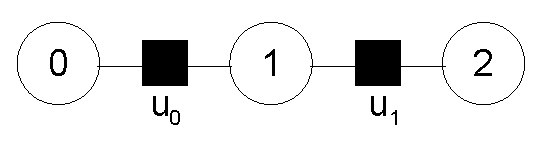
\includegraphics[width=0.7\columnwidth]{chain.pdf}
%\caption{A 0101-Chain instance of length 3.}
%\label{fig:chain}
%\end{figure}

The 0101-Chain is a simple MAMAB, %with a limited induced width (specifically $1$),
with a known optimal action. The problem consists of $n$ agents, and $n-1$ local reward functions.
Each local reward function $f^i(a_i, a_{i+1})$ is connected to the agent with the same index, $i$,
and to $i+1$. %(see Figure\ref{fig:chain}), i.e., agents $i$ and $i\!+\!1$.

\newcolumntype{x}[1]{>{\centering\arraybackslash\hspace{0pt}}p{#1}}

\begin{table}[!ht]
\begin{center}
\begin{tabular}{| l | | c | c | }
 \hline
   {\it $i$ is even} & ${a}_{i+1}=0$ & ${a}_{i+1}=1$ \\ \hline\hline
  ${a}_i =0$ & $\frac{f(\mathtt{suc};0.75)}{n-1} $   &  $\frac{1}{n-1}$ \\ \hline
  ${a}_i =1$ & $\frac{f(\mathtt{suc};0.25)}{n-1} $ &  $\frac{f(\mathtt{suc};0.9)}{n-1} $ \\ \hline
\end{tabular}
% \vskip 10pt
% \begin{tabular}{| l | | c | c | }
%  \hline
%    {\it $i$ is odd} & ${a}_{i+1}=0$ & ${a}_{i+1}=1$ \\ \hline\hline
%   ${a}_i =0$ & $\frac{f(\mathtt{suc};0.75)}{n-1} $   &  $\frac{f(\mathtt{suc};0.25)}{n-1}$ \\ \hline
%   ${a}_i =1$ & $\frac{1}{n-1} $ &  $\frac{f(\mathtt{suc};0.9)}{n-1} $ \\ \hline
% \end{tabular}
\end{center}
\caption{
The reward table for 0101-Chain. $n$ is the number of agents
in the problem. $f(\mathtt{suc};p)$ is a Bernoulli distribution with success probability
$p$, i.e., $f(1;p) = p$ and $f(0;p) = 1\!-\!p$. The table for odd agents is the same but
transposed.}
\label{tab:0101}
\end{table}

The optimal action in the 0101-Chain problem is $a_i = 0$ if $i$ is even, and $a_i = 1$ is $i$ is
odd. The reward tables for each local group are given in Table \ref{tab:0101}.

\subsection{Gem Mining}

%Gems are very rare finds, so Bernoulli bandits with low probabilities are reasonable approximation to model mining for gems.

\begin{figure}[!ht]
\centering
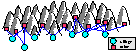
\includegraphics[width=0.88\columnwidth]{minesImg.pdf}
\caption{Gem Mining example. Each village represents an agent, while the mines represent the local
reward functions.}
\label{fig:mining}
\end{figure}

Our Gem Mining problem is adapted from the Mining Day problem from \cite{roijers2015computing},
which is a multi-objective coordination graph benchmark problem.

% While keeping the structure of Mining Day, Gem Mining has only one objective, and more importantly, a stochastic reward function rather than a deterministic one in order to create an interesting learning problem. This stochastic reward function consists of local reward functions using Bernoulli distributions with very low success probabilities. As gems are very rare finds this corresponds well to this setting, and we thus call this problem Gem Mining.

In Gem Mining, a mining company mines gems from a set of mines (local reward functions) located in
the mountains (see Figure \ref{fig:mining}). The mine workers live in villages at the foot of the
mountains. The company has one van in each village (agents) for transporting workers and must
determine every morning to which mine each van should go (actions), but vans can only travel
to nearby mines (graph connectivity).
Workers are more efficient when there are more workers at a mine: the probability of finding a gem
in a mine is $x \cdot 1.03^{w-1}$, where $x$ is the base probability of finding a gem in a mine and
$w$ is the number of workers at the mine.  To generate an instance with $v$ villages (agents), we
randomly assign 1-5 workers to each village and connect it to 2--4 mines. Each village is only
connected to mines with a greater or equal index, i.e., if village $i$ is connected to $m$ mines, it
is connected to mines $i$ to $i+m-1$. The last village is connected to $4$ mines and thus the number
of mines is $v+3$.

\subsection{Wind Farm}\label{sec:wind}

\begin{figure}[!ht]
\centering
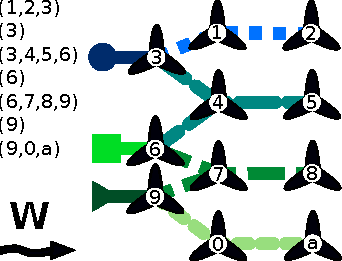
\includegraphics[width=0.7\columnwidth]{wind.pdf}
\caption{Wind farm setup. The incoming wind is denoted by an arrow. Each local group is denoted by a
different color and line type. Groups are listed explicitly on the left. Note the three single-agent
groups on the left to handle per-agent rewards.}
\label{fig:wind_graph}
\end{figure}

In our wind farm experiment, we used a state-of-the-art simulator \cite{vandijk2016} to mimic the energy production of a series of wind turbines when exposed to a global incoming wind vector. In the real world, turbines can often be oriented at certain angles to maximize production. This is a non-trivial control task, as the turbulence caused by a turbine will negatively affect turbines downwind. The direction of this generated turbulence depends on the angle that the turbine has w.r.t. the incoming wind vector.

We setup our simulated wind farm using 11 turbines (see Figure~\ref{fig:wind_graph}). Each turbine has a
choice between three different actions (angles) that it can turn to. The last $4$ turbines downwind (2, 5, 8, and $a$)
are set directly against the wind and are not controlled by agents, as they cannot generate
turbulence that can impact power production. However, the remaining $7$ turbines do influence the
rest of the farm, and so must cooperate to maximize power production.

\begin{figure*}[ht!]
\centering
\subfigure[0101-Chain, All Algorithms]{\label{fig:nodes_all}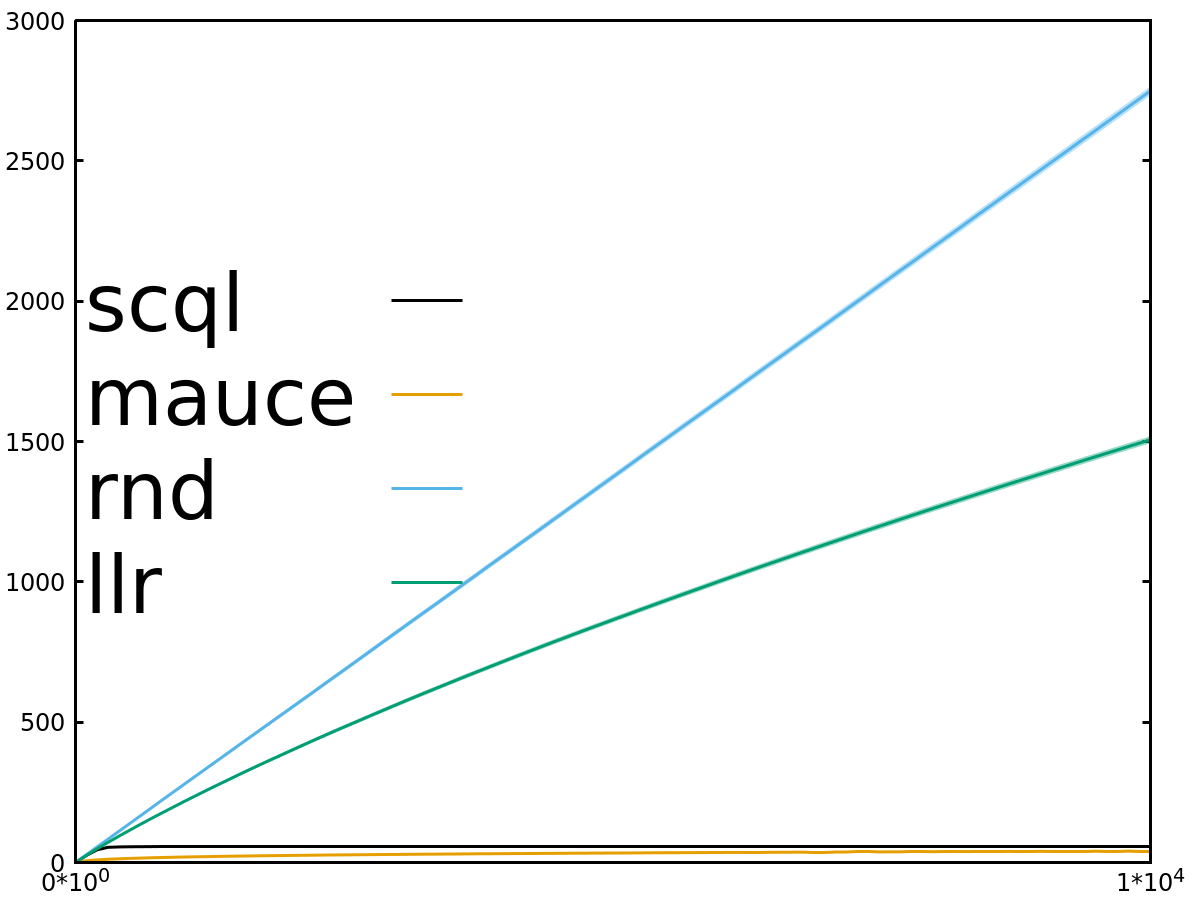
\includegraphics[width=0.49\columnwidth]{nodes_all.png}}
\subfigure[0101-Ch., MAUCE\&SCQL]{\label{fig:nodes_xs}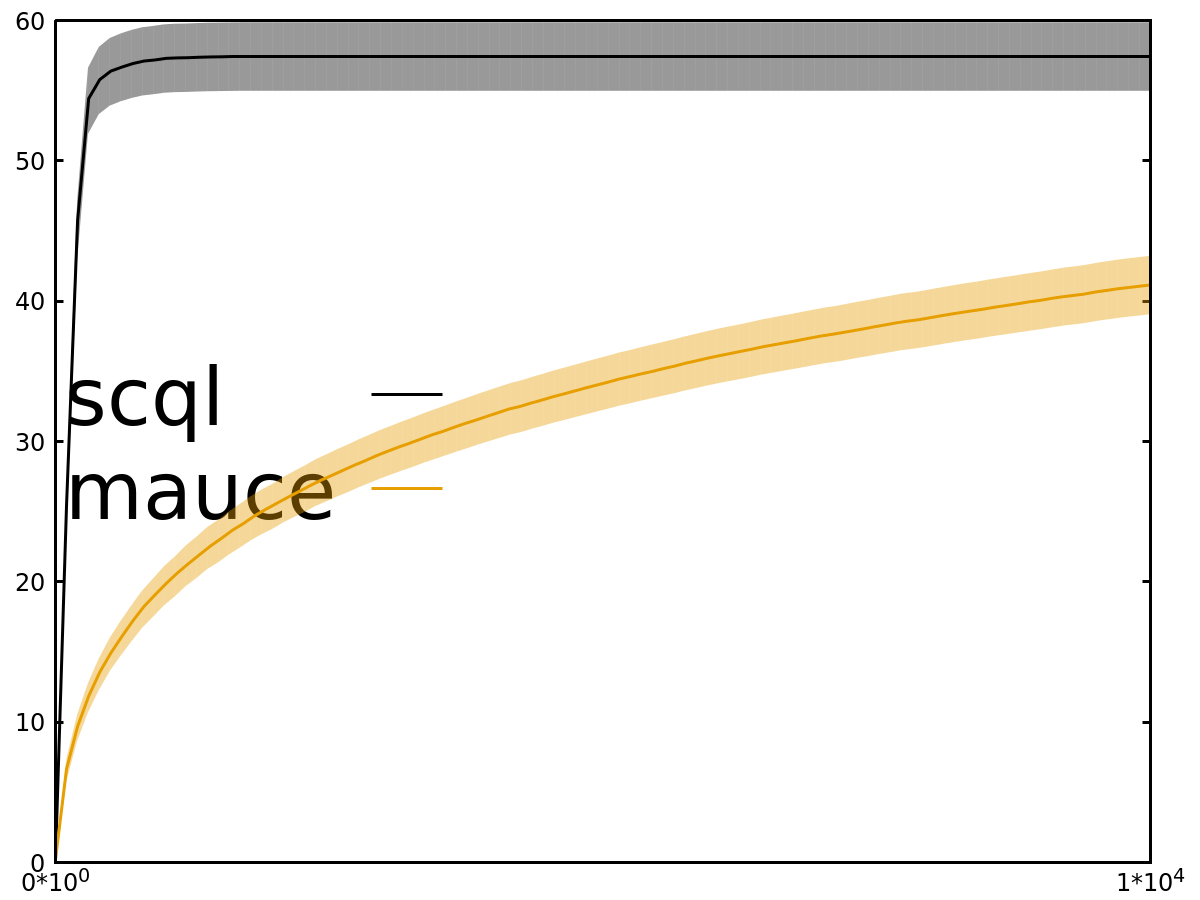
\includegraphics[width=0.49\columnwidth]{nodes_xs.png}}
\subfigure[Gem Mining]{\label{fig:mines}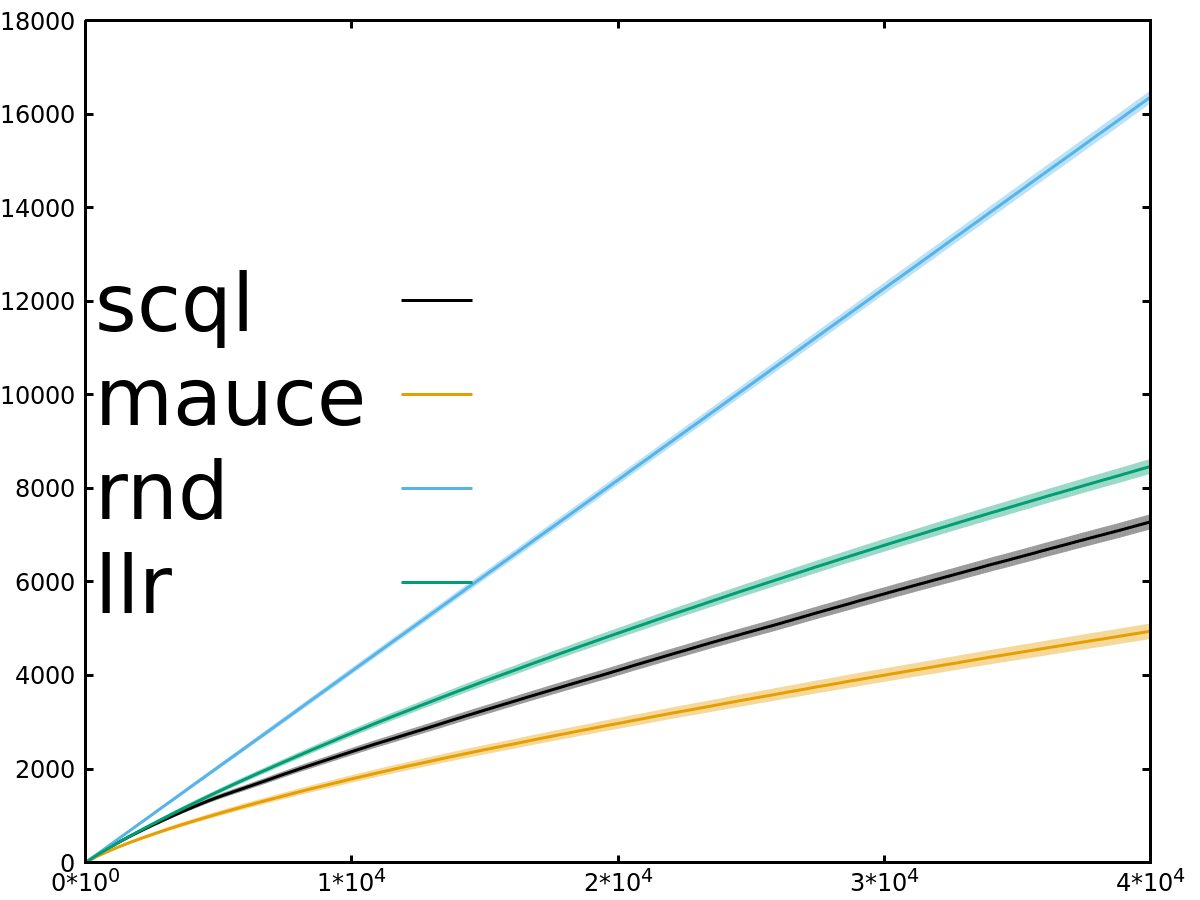
\includegraphics[width=0.49\columnwidth]{mines.png}}
\subfigure[Wind Farm]{\label{fig:wind}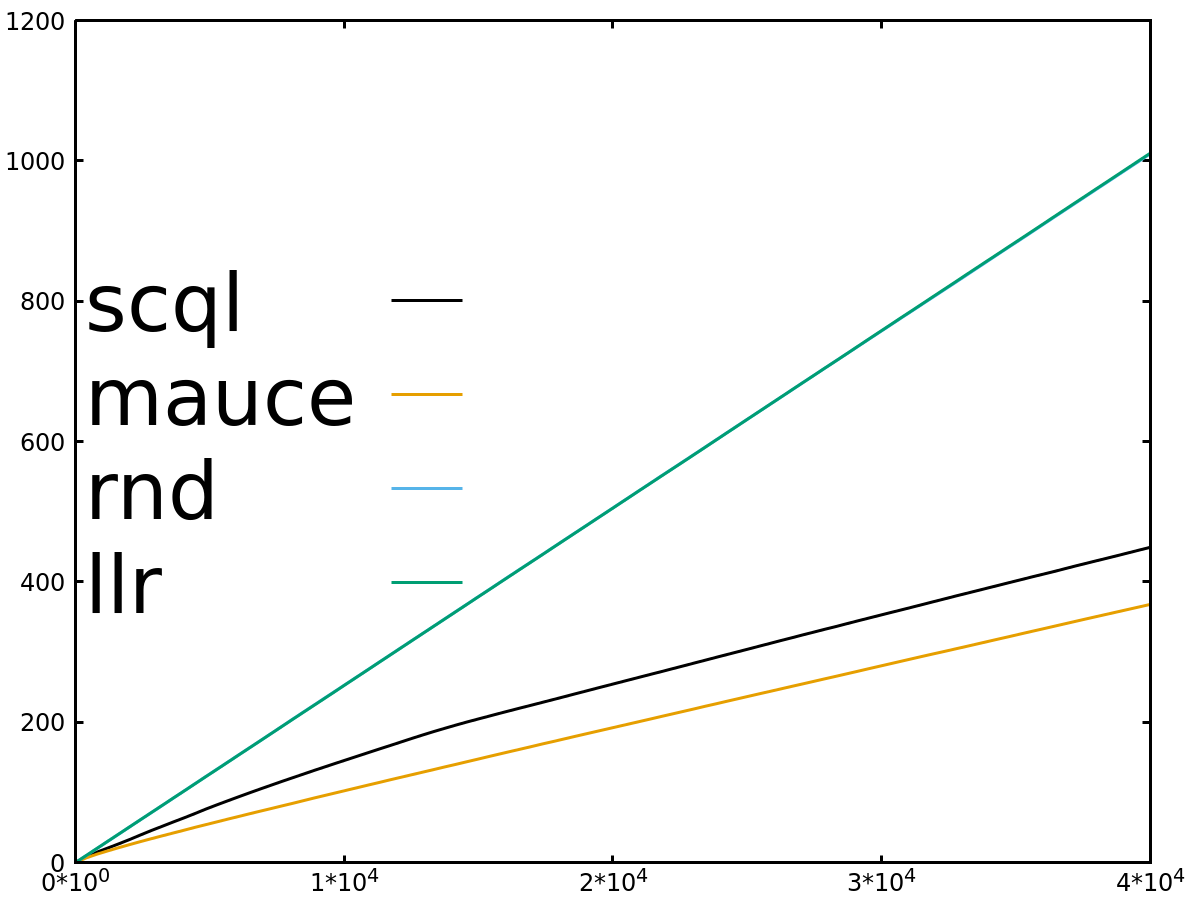
\includegraphics[width=0.49\columnwidth]{wind.png}}
%\subfigure[0101-Chain, All Algorithms]{\label{fig:nodes_all}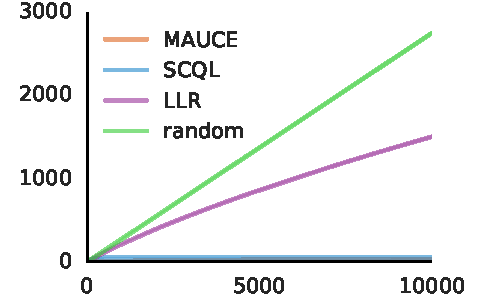
\includegraphics[width=0.49\columnwidth]{nodes1.pdf}}
%\subfigure[0101-Ch., MAUCE\&SCQL]{\label{fig:nodes_xs}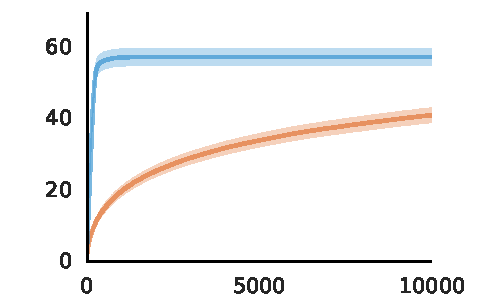
\includegraphics[width=0.49\columnwidth]{nodes2.pdf}}
%\subfigure[Gem Mining]{\label{fig:mines}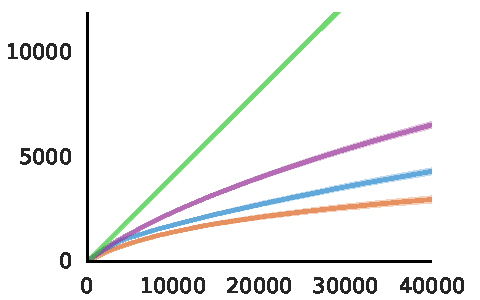
\includegraphics[width=0.49\columnwidth]{mines3.pdf}}
%\subfigure[Wind Farm]{\label{fig:wind}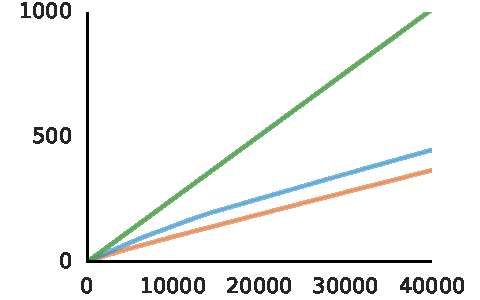
\includegraphics[width=0.49\columnwidth]{wind4.pdf}}
\caption{Cumulative regret for all experiments as a function of the number of actions executed: a)
0101-Chain averaged over 100 runs, b) Same as \ref{fig:nodes_all}, only SCQL and MAUCE, c) Gem
Mining, averaged over 5 random setups, 100 runs per setup, and d) Wind Farm, 10 runs. }
\label{fig:nodes_results}
\end{figure*}

We vary the wind speed in the simulator at each timestep, following a truncated normal distribution
with mean $8.1$ m/s. The overall reward is normalized to a $[0, 1]$ interval using the maximum
possible overall reward at the highest wind strength and the minimum possible reward per turbine at
the minimum wind strength. While this makes it impossible to compute the true regret, as choosing
the optimal action does not result in a $0$ regret in expectation, it avoids having to calculate the
true expected reward for all actions in this scenario, which is non-trivial.

Differently from the previous experiments, rewards in this settings are obtained per-agent from the
simulator rather than per-group. Thus, we use single-agent local groups to prevent dependencies
between the reward functions of each group. The reward for agents in more than one group is given
solely to their single-agent group, and none to the others (rather than splitting).

\subsection{Results}

We tested the performance of MAUCE on the higly structured 0101-Chain problem with 11 agents for
10,000 joint action executions, and compare its performance against random, SCQL and LLR. The
results (Figure \ref{fig:nodes_results}) indicate that both SCQL and MAUCE can learn effectively,
far outclassing random joint action selection and LLR.

When comparing MAUCE and SCQL (Figure \ref{fig:nodes_xs}), MAUCE achieves considerably less regret than SCQL. This is because MAUCE's exploration strategy is based on the aggregation of local exploration bounds, while SCQL uses an $\varepsilon$-greedy exploration strategy. On the other hand, SCQL does learn the optimal joint action quickly, thanks to optimistic initialization and this aggressive exploration strategy. We note that after a while, we decreased $\varepsilon$ to $0$, i.e., only exploit, making the regret graph a flat line from that point onward. We note that the annealing of $\varepsilon$ needed to be fine-tuned.
We thus conclude that MAUCE is an effective algorithm that can exploit the graphical structure, leading to superior performance for this highly-structured problem.

We then tested MAUCE against the other algorithms on randomly generated Gem Mining instances with 5
villages and 8 mines, to compare performances on a more challenging problem. Figure \ref{fig:mines}
represents the average regret over multiple different scenarios. We observe that, while SCQL and LLR
are all able to achieve sublinear regret curves, MAUCE handles the exploration-exploitation
tradeoffs best, resulting in the lowest regret over time.

Finally, to test the performance of MAUCE on a real-world problem, we run the algorithms on a Wind
Farm instance (Figure \ref{fig:wind}). Due to the high computational costs of running the simulator,
we perform only ten runs. As explained before, the measure shown is not an exact form of regret, as
the optimal action will not result in a $0$ regret in expectation.

The MAUCE algorithm once again performs best, with less cumulative regret than both LLR and SCQL.
The LLR algorithm also doesn't seem to achieve any significant learning with respect to the random
policy. Note that MAUCE keeps learning and fine tuning this policy over the whole duration of the
experiment, which allows it to increasingly achieve lower regret than SCQL. At timestep 10000, the
difference between the two is $43.258$, while at timestep 40000 it is $81.373$.  It is important to
note that SCQL could probably be made to perform better by finely tuning the initialization values
and epsilon updates, but this would take significant human time and repetitive trials. MAUCE can
instead directly manage the exploration-exploitation trade-off by using its local bounds for each
local joint action.

We thus conclude that MAUCE is an effective algorithm for trading off exploration versus exploitation in MAMABs, and has superior performance w.r.t.\ the alternative algorithms.

 %SCQL on the other hand, while it can be less performant due to the difficulty of correctly setting up its exploration methods, can be more resilient when dealing with unknown problems as it is harder to mess up optimistic initialization and an epsilon policy.

%\textcolor{blue}{(Timo: how many times have these experiments been run?)}


\section{Conclusion}
In this paper, we proposed the \emph{multi-agent upper confidence exploration (MAUCE)} algorithm for \emph{multi-agent multi-armed bandits (MAMABs)}. MAUCE exploits the graphical properties of the MAMAB in a reinforcement learning setting, by treating exploitation, i.e., the sum over estimated mean local rewards, and exploitation, expressed as a function of the sum over weighted inverse local counts, as separate objectives. Via a subroutine, \emph{upper confidence variable elimination (UCVE)}, that can handle these objectives, MAUCE selects the action that best balances exploration  and exploitation according to the joint overall mean reward plus (upper confidence) exploration bound. We have proven a regret bound for MAUCE that is only linear in the number of agents, rather than exponential, as it would be if we were to flatten the MAMAB to a single-agent MAB. Furthermore, the regret bound is logarithmic in the number of arm pulls. 
We compared MAUCE empirically to state-of-the-art algorithms in multi-agent reinforcement learning and combinatorial bandits, and have shown that MAUCE achieves much lower in-practice regret than these approaches.

In future work, we aim to build on MAUCE to achieve quality guarantees for reinforcement learning in multi-agent MDPs, in addition to the bounds for MAMABs we have proven in this paper. 

\bibliography{dmrThesis}
\bibliographystyle{icml2018}


%%%%%%%%%%%%%%%%%%%%%%%%%%%%%%%%%%%%%%%%%%%%%%%%%%%%%%%%%%%%%%%%%%%%%%%%%%%%%%%
%%%%%%%%%%%%%%%%%%%%%%%%%%%%%%%%%%%%%%%%%%%%%%%%%%%%%%%%%%%%%%%%%%%%%%%%%%%%%%%
% DELETE THIS PART. DO NOT PLACE CONTENT AFTER THE REFERENCES!
%%%%%%%%%%%%%%%%%%%%%%%%%%%%%%%%%%%%%%%%%%%%%%%%%%%%%%%%%%%%%%%%%%%%%%%%%%%%%%%
%%%%%%%%%%%%%%%%%%%%%%%%%%%%%%%%%%%%%%%%%%%%%%%%%%%%%%%%%%%%%%%%%%%%%%%%%%%%%%%
%\appendix
%%%%%%%%%%%%%%%%%%%%%%%%%%%%%%%%%%%%%%%%%%%%%%%%%%%%%%%%%%%%%%%%%%%%%%%%%%%%%%%
%%%%%%%%%%%%%%%%%%%%%%%%%%%%%%%%%%%%%%%%%%%%%%%%%%%%%%%%%%%%%%%%%%%%%%%%%%%%%%%


\end{document}


% This document was modified from the file originally made available by
% Pat Langley and Andrea Danyluk for ICML-2K. This version was created
% by Iain Murray in 2018. It was modified from a version from Dan Roy in
% 2017, which was based on a version from Lise Getoor and Tobias
% Scheffer, which was slightly modified from the 2010 version by
% Thorsten Joachims & Johannes Fuernkranz, slightly modified from the
% 2009 version by Kiri Wagstaff and Sam Roweis's 2008 version, which is
% slightly modified from Prasad Tadepalli's 2007 version which is a
% lightly changed version of the previous year's version by Andrew
% Moore, which was in turn edited from those of Kristian Kersting and
% Codrina Lauth. Alex Smola contributed to the algorithmic style files.
